\documentclass[12pt, a4paper, Spanish]{article}
\usepackage[utf8]{inputenc}
\usepackage{
    graphicx,
    enumitem,
    chngcntr,
    csquotes,
    amsmath,
    mathptmx,
    amssymb,
    float,
    amssymb,
    amsfonts,
    fullpage,
    caption
}
\usepackage{hyperref}
\usepackage{xcolor}
\hypersetup{colorlinks=true, linkcolor=black, urlcolor=cyan, citecolor=black}
\graphicspath{{imagenes/}}

\begin{document}

\section*{Resultados}

\begin{figure}[H]
    \centering
    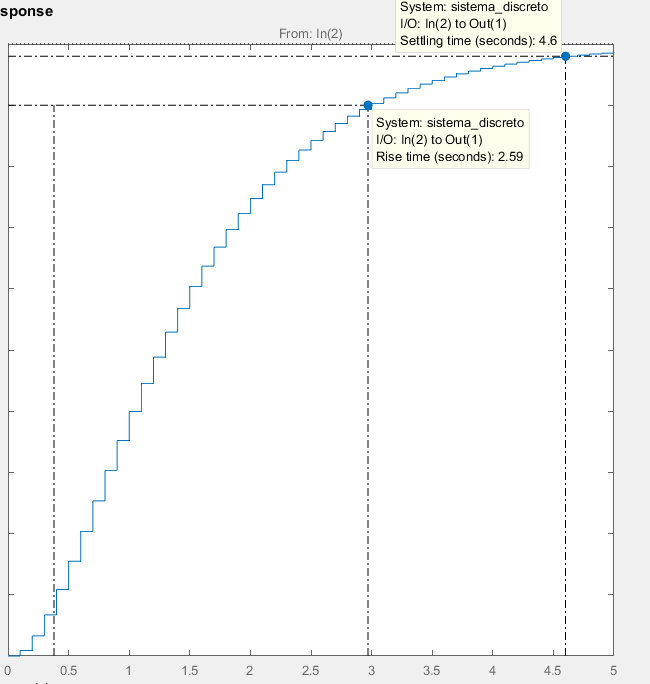
\includegraphics[width=0.7\textwidth]{respuesta-en-tiempo-sistema-lazo-abierto.png}
    \caption{Respuesta en tiempo del sistema en lazo abierto.}
    \label{fig:lazo_abierto}
\end{figure}

\begin{figure}[H]
    \centering
    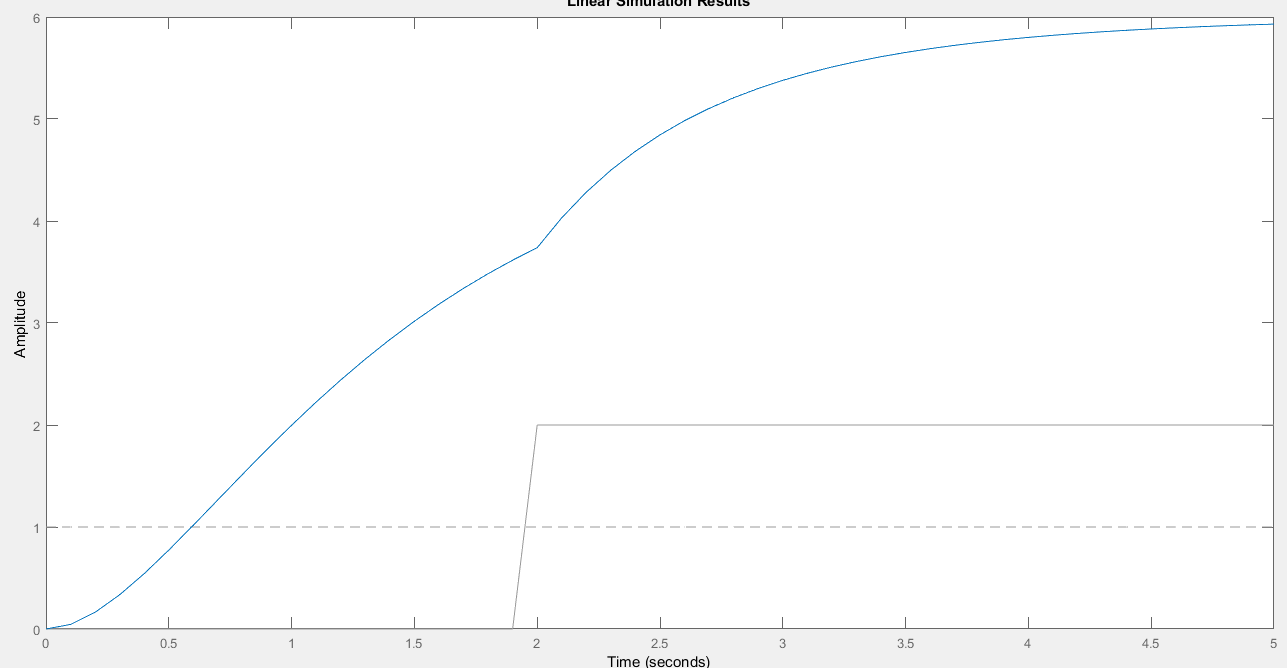
\includegraphics[width=0.8\textwidth]{respuesta-en-tiempo-sistema-lazo-abierto-con-perturbacion.png}
    \caption{Respuesta en tiempo del sistema en lazo abierto con perturbación en t=2.}
    \label{fig:lazo_abierto_perturbacion}
\end{figure}

\begin{figure}[H]
    \centering
    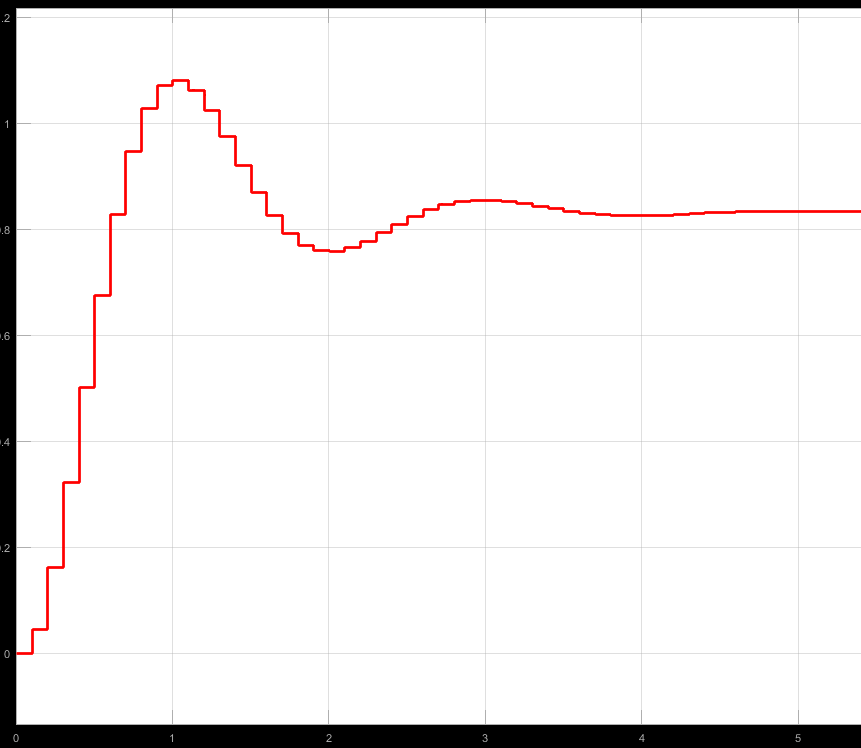
\includegraphics[width=0.5\textwidth]{respuesta-en-tiempo-sistema-lazo-cerrado-1.png}
    \caption{Respuesta en tiempo del sistema en lazo cerrado (Kp=1, Ki=0, Kd=0, Td=0).}
    \label{fig:lazo_cerrado_1}
\end{figure}

\begin{figure}[H]
    \centering
    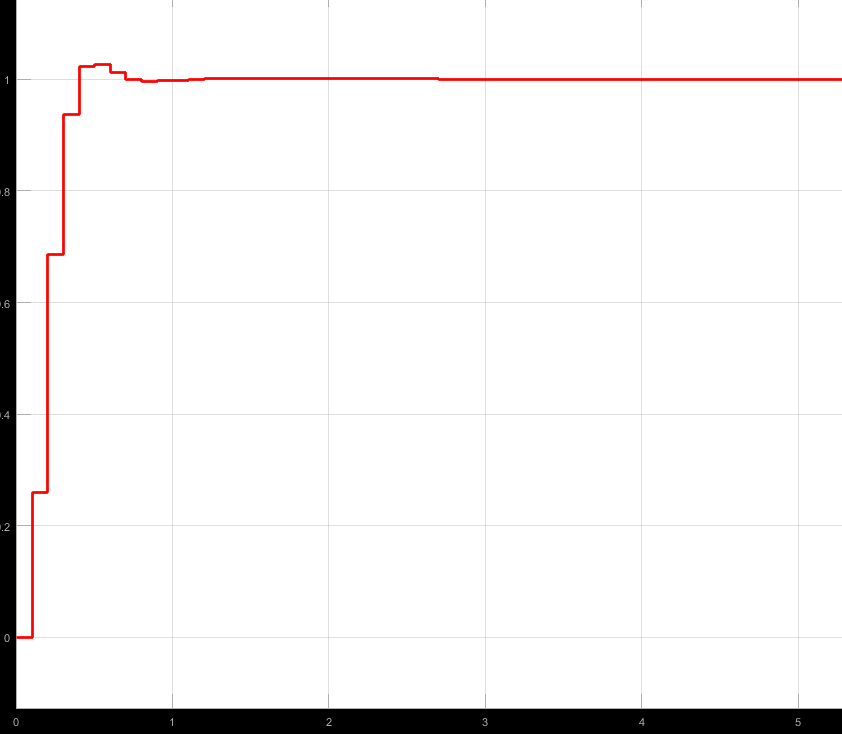
\includegraphics[width=0.5\textwidth]{respuesta-en-tiempo-sistema-lazo-cerrado-2.png}
    \caption{Respuesta en tiempo del sistema en lazo cerrado (Kp=1.45, Ki=1, Kd=0.43, Td=0).}
    \label{fig:lazo_cerrado_2}
\end{figure}

\begin{figure}[H]
    \centering
    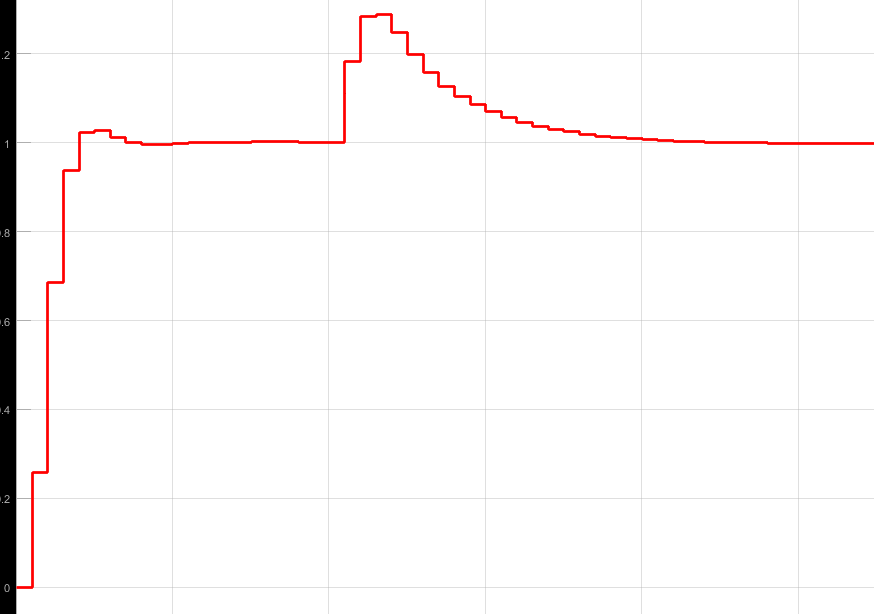
\includegraphics[width=0.5\textwidth]{respuesta-en-tiempo-sistema-lazo-cerrado-3.png}
    \caption{Respuesta en tiempo del sistema en lazo cerrado (Kp=1.45, Ki=1, Kd=0.43, Td=1).}
    \label{fig:lazo_cerrado_3}
\end{figure}

\end{document}
